\section{Hardware Support}

The embedded world use the majority of the world's microcontrollers.
The diversity of CPU keep increasing every year.
Working with this diversity of constrained devices make the developer's work harder as he need to adapt and learn to use specific librairies for each devices.
A source code on a particular device will not be easily reusable for another device.

With RTOSes, developers can more easily make their code portable on many devices.

This section first describes the three constrained devices classes and how this is related to RTOSes.
Then, it explains what an hardware abstraction layer is and how a RTOS use it in order to be available on the largest amount of devices.

\subsection{Constrained devices classes}

Constrained devices have been classified in 3 classes by the IETF with RFC7228 in May 2014. The distinction between those three classes are made with the RAM and ROM capabilities.
The table \ref{tab:constrained-devices-classes} resumes the different constrained devices classes.

\begin{table}[!h]
  \centering
  \begin{tabular}{|l|l|l|}
  \hline
   & data size (e.g., RAM) & code size (e.g., Flash) \\ \hline
  Class 0, C0 & \textless{}\textless{} 10 KiB & \textless{}\textless{} 100 KiB \\ %\hline
  Class 1, C1 & $\sim$ 10 Kib & $\sim$ 100 KiB \\ %\hline
  Class 2, C2 & $\sim$ 50 KiB & $\sim$ 250 KiB \\ \hline
  \end{tabular}
  \caption{Classes of Constrained Devices}
  \label{tab:constrained-devices-classes}
\end{table}

\paragraph{Class 0}
Those devices are the most constrained.
There are typically sensor-like motes.
There are so constrained that they cannot access Internet without the help of a larger devices.
From the point of view of a RTOS, their code are too heavy to fit in such devices.
Instead Class-0 devices are usually used bare metal.
In the embedded world, bare metal programming is writing code that runs directly on the hardware without any abstraction such as an OS.

\paragraph{Class 1}
Those devices are able to talk to each other but via constrained protocols.
Use of security protocols are too heavy for that class.
RTOS are mainly focused on these kind of devices.

\paragraph{Class 2}
Those devices are the less constrained and can use the same stacks of protocols used in personal computers and servers.
General-purpose operating systems can be used for these kind of devices but the Class-2 devices can benefit from lightweight and energy-efficient protocols.

\subsection{Hardware Abstraction Layer}

Due to the variety of CPU's, vendors provide a set of libraires used to develop applications on their architectures.
This set of libraires and tools are called the hardware abstraction layer.

\paragraph{Definition of HAL}
% TODO
% Repetition of 'hardware'
An hardware abstraction layer defines a set of routines, protocols and tools to access underlying hardware.
It provides abstract and high-level functions to interact with the hardware.
The hardware, drivers and board supports are considered as a black-box.

\paragraph{RTOS and HAL}
The HAL is strongly dependent of the architecture of the CPU.
In order for the RTOS to support multiple boards and architectures, it has to implement and use the different HAL provided by the vendors.

\begin{figure}[!h]
  \centering
  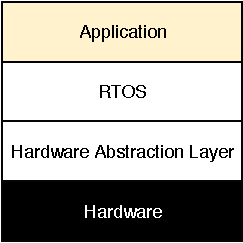
\includegraphics[scale=1]{assets/hal-layers.pdf}
  \caption{\label{fig:hal-layer}Layers around the hardware abstraction layer}
\end{figure}

The figure \ref{fig:hal-layer} shows that the application and the RTOS layers are placed above the HAL, itself just above the device layer.
The application layer talks to the RTOS and the RTOS layer talks to the corresponding HAL depending on the device used.


\paragraph{Pro and cons}
Developers can switch hardware and perform cross-platform testing more easily.
But there is some limitation: The HAL is tied to the hardware and change heavily with it.
Also, there is some limitation using an hardware abstraction layer.
Not all the functionalities from the hardware are available.